% Options for packages loaded elsewhere
\PassOptionsToPackage{unicode}{hyperref}
\PassOptionsToPackage{hyphens}{url}
%
\documentclass[
  12pt,
]{article}
\usepackage{amsmath,amssymb}
\usepackage{iftex}
\ifPDFTeX
  \usepackage[T1]{fontenc}
  \usepackage[utf8]{inputenc}
  \usepackage{textcomp} % provide euro and other symbols
\else % if luatex or xetex
  \usepackage{unicode-math} % this also loads fontspec
  \defaultfontfeatures{Scale=MatchLowercase}
  \defaultfontfeatures[\rmfamily]{Ligatures=TeX,Scale=1}
\fi
\usepackage{lmodern}
\ifPDFTeX\else
  % xetex/luatex font selection
    \setmainfont[]{Times New Roman}
\fi
% Use upquote if available, for straight quotes in verbatim environments
\IfFileExists{upquote.sty}{\usepackage{upquote}}{}
\IfFileExists{microtype.sty}{% use microtype if available
  \usepackage[]{microtype}
  \UseMicrotypeSet[protrusion]{basicmath} % disable protrusion for tt fonts
}{}
\makeatletter
\@ifundefined{KOMAClassName}{% if non-KOMA class
  \IfFileExists{parskip.sty}{%
    \usepackage{parskip}
  }{% else
    \setlength{\parindent}{0pt}
    \setlength{\parskip}{6pt plus 2pt minus 1pt}}
}{% if KOMA class
  \KOMAoptions{parskip=half}}
\makeatother
\usepackage{xcolor}
\usepackage[margin=1in]{geometry}
\usepackage{color}
\usepackage{fancyvrb}
\newcommand{\VerbBar}{|}
\newcommand{\VERB}{\Verb[commandchars=\\\{\}]}
\DefineVerbatimEnvironment{Highlighting}{Verbatim}{commandchars=\\\{\}}
% Add ',fontsize=\small' for more characters per line
\usepackage{framed}
\definecolor{shadecolor}{RGB}{248,248,248}
\newenvironment{Shaded}{\begin{snugshade}}{\end{snugshade}}
\newcommand{\AlertTok}[1]{\textcolor[rgb]{0.94,0.16,0.16}{#1}}
\newcommand{\AnnotationTok}[1]{\textcolor[rgb]{0.56,0.35,0.01}{\textbf{\textit{#1}}}}
\newcommand{\AttributeTok}[1]{\textcolor[rgb]{0.13,0.29,0.53}{#1}}
\newcommand{\BaseNTok}[1]{\textcolor[rgb]{0.00,0.00,0.81}{#1}}
\newcommand{\BuiltInTok}[1]{#1}
\newcommand{\CharTok}[1]{\textcolor[rgb]{0.31,0.60,0.02}{#1}}
\newcommand{\CommentTok}[1]{\textcolor[rgb]{0.56,0.35,0.01}{\textit{#1}}}
\newcommand{\CommentVarTok}[1]{\textcolor[rgb]{0.56,0.35,0.01}{\textbf{\textit{#1}}}}
\newcommand{\ConstantTok}[1]{\textcolor[rgb]{0.56,0.35,0.01}{#1}}
\newcommand{\ControlFlowTok}[1]{\textcolor[rgb]{0.13,0.29,0.53}{\textbf{#1}}}
\newcommand{\DataTypeTok}[1]{\textcolor[rgb]{0.13,0.29,0.53}{#1}}
\newcommand{\DecValTok}[1]{\textcolor[rgb]{0.00,0.00,0.81}{#1}}
\newcommand{\DocumentationTok}[1]{\textcolor[rgb]{0.56,0.35,0.01}{\textbf{\textit{#1}}}}
\newcommand{\ErrorTok}[1]{\textcolor[rgb]{0.64,0.00,0.00}{\textbf{#1}}}
\newcommand{\ExtensionTok}[1]{#1}
\newcommand{\FloatTok}[1]{\textcolor[rgb]{0.00,0.00,0.81}{#1}}
\newcommand{\FunctionTok}[1]{\textcolor[rgb]{0.13,0.29,0.53}{\textbf{#1}}}
\newcommand{\ImportTok}[1]{#1}
\newcommand{\InformationTok}[1]{\textcolor[rgb]{0.56,0.35,0.01}{\textbf{\textit{#1}}}}
\newcommand{\KeywordTok}[1]{\textcolor[rgb]{0.13,0.29,0.53}{\textbf{#1}}}
\newcommand{\NormalTok}[1]{#1}
\newcommand{\OperatorTok}[1]{\textcolor[rgb]{0.81,0.36,0.00}{\textbf{#1}}}
\newcommand{\OtherTok}[1]{\textcolor[rgb]{0.56,0.35,0.01}{#1}}
\newcommand{\PreprocessorTok}[1]{\textcolor[rgb]{0.56,0.35,0.01}{\textit{#1}}}
\newcommand{\RegionMarkerTok}[1]{#1}
\newcommand{\SpecialCharTok}[1]{\textcolor[rgb]{0.81,0.36,0.00}{\textbf{#1}}}
\newcommand{\SpecialStringTok}[1]{\textcolor[rgb]{0.31,0.60,0.02}{#1}}
\newcommand{\StringTok}[1]{\textcolor[rgb]{0.31,0.60,0.02}{#1}}
\newcommand{\VariableTok}[1]{\textcolor[rgb]{0.00,0.00,0.00}{#1}}
\newcommand{\VerbatimStringTok}[1]{\textcolor[rgb]{0.31,0.60,0.02}{#1}}
\newcommand{\WarningTok}[1]{\textcolor[rgb]{0.56,0.35,0.01}{\textbf{\textit{#1}}}}
\usepackage{longtable,booktabs,array}
\usepackage{calc} % for calculating minipage widths
% Correct order of tables after \paragraph or \subparagraph
\usepackage{etoolbox}
\makeatletter
\patchcmd\longtable{\par}{\if@noskipsec\mbox{}\fi\par}{}{}
\makeatother
% Allow footnotes in longtable head/foot
\IfFileExists{footnotehyper.sty}{\usepackage{footnotehyper}}{\usepackage{footnote}}
\makesavenoteenv{longtable}
\usepackage{graphicx}
\makeatletter
\def\maxwidth{\ifdim\Gin@nat@width>\linewidth\linewidth\else\Gin@nat@width\fi}
\def\maxheight{\ifdim\Gin@nat@height>\textheight\textheight\else\Gin@nat@height\fi}
\makeatother
% Scale images if necessary, so that they will not overflow the page
% margins by default, and it is still possible to overwrite the defaults
% using explicit options in \includegraphics[width, height, ...]{}
\setkeys{Gin}{width=\maxwidth,height=\maxheight,keepaspectratio}
% Set default figure placement to htbp
\makeatletter
\def\fps@figure{htbp}
\makeatother
\setlength{\emergencystretch}{3em} % prevent overfull lines
\providecommand{\tightlist}{%
  \setlength{\itemsep}{0pt}\setlength{\parskip}{0pt}}
\setcounter{secnumdepth}{5}
% definitions for citeproc citations
\NewDocumentCommand\citeproctext{}{}
\NewDocumentCommand\citeproc{mm}{%
  \begingroup\def\citeproctext{#2}\cite{#1}\endgroup}
\makeatletter
 % allow citations to break across lines
 \let\@cite@ofmt\@firstofone
 % avoid brackets around text for \cite:
 \def\@biblabel#1{}
 \def\@cite#1#2{{#1\if@tempswa , #2\fi}}
\makeatother
\newlength{\cslhangindent}
\setlength{\cslhangindent}{1.5em}
\newlength{\csllabelwidth}
\setlength{\csllabelwidth}{3em}
\newenvironment{CSLReferences}[2] % #1 hanging-indent, #2 entry-spacing
 {\begin{list}{}{%
  \setlength{\itemindent}{0pt}
  \setlength{\leftmargin}{0pt}
  \setlength{\parsep}{0pt}
  % turn on hanging indent if param 1 is 1
  \ifodd #1
   \setlength{\leftmargin}{\cslhangindent}
   \setlength{\itemindent}{-1\cslhangindent}
  \fi
  % set entry spacing
  \setlength{\itemsep}{#2\baselineskip}}}
 {\end{list}}
\usepackage{calc}
\newcommand{\CSLBlock}[1]{\hfill\break\parbox[t]{\linewidth}{\strut\ignorespaces#1\strut}}
\newcommand{\CSLLeftMargin}[1]{\parbox[t]{\csllabelwidth}{\strut#1\strut}}
\newcommand{\CSLRightInline}[1]{\parbox[t]{\linewidth - \csllabelwidth}{\strut#1\strut}}
\newcommand{\CSLIndent}[1]{\hspace{\cslhangindent}#1}
\usepackage{tcolorbox}
\usepackage{amssymb}
\usepackage{yfonts}
\usepackage{bm}
\usepackage{titlesec}
\usepackage{kbordermatrix}


\newtcolorbox{greybox}{
  colback=white,
  colframe=blue,
  coltext=black,
  boxsep=5pt,
  arc=4pt}
  
\newcommand{\sectionbreak}{\clearpage}

 
\newcommand{\ds}[4]{\sum_{{#1}=1}^{#3}\sum_{{#2}=1}^{#4}}
\newcommand{\us}[3]{\mathop{\sum\sum}_{1\leq{#2}<{#1}\leq{#3}}}

\newcommand{\ol}[1]{\overline{#1}}
\newcommand{\ul}[1]{\underline{#1}}

\newcommand{\amin}[1]{\mathop{\text{argmin}}_{#1}}
\newcommand{\amax}[1]{\mathop{\text{argmax}}_{#1}}

\newcommand{\ci}{\perp\!\!\!\perp}

\newcommand{\mc}[1]{\mathcal{#1}}
\newcommand{\mb}[1]{\mathbb{#1}}
\newcommand{\mf}[1]{\mathfrak{#1}}

\newcommand{\eps}{\epsilon}
\newcommand{\lbd}{\lambda}
\newcommand{\alp}{\alpha}
\newcommand{\df}{=:}
\newcommand{\am}[1]{\mathop{\text{argmin}}_{#1}}
\newcommand{\ls}[2]{\mathop{\sum\sum}_{#1}^{#2}}
\newcommand{\ijs}{\mathop{\sum\sum}_{1\leq i<j\leq n}}
\newcommand{\jis}{\mathop{\sum\sum}_{1\leq j<i\leq n}}
\newcommand{\sij}{\sum_{i=1}^n\sum_{j=1}^n}
	
\ifLuaTeX
  \usepackage{selnolig}  % disable illegal ligatures
\fi
\usepackage{bookmark}
\IfFileExists{xurl.sty}{\usepackage{xurl}}{} % add URL line breaks if available
\urlstyle{same}
\hypersetup{
  pdfauthor={Jan de Leeuw - University of California Los Angeles},
  hidelinks,
  pdfcreator={LaTeX via pandoc}}

\title{Smacof at 50: A Manual\\
Part 4: Smacof for Tetrads}
\author{Jan de Leeuw - University of California Los Angeles}
\date{Started May 19 2024, Version of July 01, 2024}

\begin{document}
\maketitle

{
\setcounter{tocdepth}{3}
\tableofcontents
}
\textbf{Note:} This is a working paper which will be expanded/updated
frequently. All suggestions for improvement are welcome. All Rmd, tex,
html, pdf, R, and C files are in the public domain. Attribution will be
appreciated, but is not required. The files can be found at
\url{https://github.com/deleeuw} in the smacofPC directory of the
repositories smacofCode, smacofManual, and smacofExamples.

\sectionbreak

\section{Introduction}\label{introduction}

The paired comparison of pairs of objects is the simplest and
the most basic one of the cartwheel methods for collecting
similarity judgments (Coombs (1954)).
Pairs of objects from a set
\(\mathcal{O}\) of \(n\) objects are compared, and the data indicate which of the two
pairs is the most similar. Torgerson (1958) (p.~261-262) calls this the \emph{method of tetrads}, and we shall adopt this terminology by referring to a pair of pairs of objects \(((o_i,o_j),(o_k,o_l))\) as a \emph{tetrad}. This is of course not to be confused with the use of ``tetrads'' in factor analysis.

In Torgerson's method of tetrads we need replications over occasions (or subjects) to estimate the probability of the \((o_i,o_j)\lesssim (o_k,o_l)\) judgments, which can then turned into scale values using Thurstonian paired comparison methods. In the smacofPC method we discuss here no replications are needed and we can apply MDS to the data from a single occasion without replications of tetrads.

In the MDS context the response
that objects \(o_i\) and \(o_j\) are more similar than objects
\(o_k\) and \(o_l\) means that we require
of our representation \(X\) that \(d_{ij}(X)\leq d_{kl}(X)\). smacofPC()
finds an approximate solution to this highly non-linear and
highly non-convex system of inequalities.

smacofPC() is not limited to data collected as comparisons of
pairs of objects. Many different data collection methods produce data that are not directly of this form, but that can be
coded as such paired comparisons. Examples are the various versions of the
method of triads, the method of conditional rank orders, and the
complete or partial ranking of all \(\binom{n}{2}\) dissimilarities.
In general the comparison data for pairs of pairs do not require transitivity or symmetry and allow for replications of some or all pairs of pairs.

There have been earlier versions of non-metric MDS methods based
on comparisons of pairs of objects. Around 1970 various people proposed the \emph{positive orthant method (POM)} (De Leeuw (1968), De Leeuw (1970), Hartmann (1979)), the \emph{absolute value principle (AVP)} (Guttman (1969)), and the
\emph{pairwise nonmetric method (PNM)} (Johnson (1973)). Guttman's conference
presentation has been republished as Guttman (1979).

The POM, AVP, and PNM methods all use an implicitly normalized least squares loss function with a numerator of the form
\begin{equation}
\lambda_N(X):=\sum\sum w_{ij,kl}\ \sigma_{ij,kl}\ \text{sign}(d_{ij}(X)-d_{kl}(X))|d_{ij}(X)-d_{kl}(X)|^q,
\label{eq:pom}
\end{equation}
where \(w_{ij,kl}\geq 0\) and \(\sigma_{ij,kl}\) is either minus one, plus one, or
zero. In most cases \(\sigma_{ij,kl}\) is the signature of the dissimilarities, i.e.
\begin{equation}
\sigma_{ij,kl}=\text{sign}(\delta_{ij}-\delta_{kl}),
\label{eq:sijkl}
\end{equation}
but that is not necessarily the case, if only because there may not be numerical dissimilarities. It is useful, however, to keep this interpretation in mind. In Johnson's PNM squared distances instead of distances are used, but at the conceptual level that seems just a minor detail.

The denominator of the loss function in all three approaches is
\begin{equation}
\lambda_D(X):=\sum\sum w_{ij,kl}|d_{ij}(X)-d_{kl}(X))|^q,
\label{eq:lambdad}
\end{equation}
and all three algorithms use gradient methods to minimize their loss functions
\(\lambda(X)=\lambda_N(X)/\lambda_D(X)\).

In both AVP and the more recent version of POM (De Leeuw (2018)) emphasis is on
\(q=1\), in which case the loss function is
\begin{equation}
\lambda(X)=\frac{\sum\sum w_{ij,kl}\ \sigma_{ij,kl}(d_{ij}(X)-d_{kl}(X))}{\sum\sum w_{ij,kl}\ |d_{ij}(X)-d_{kl}(X)|}.
\label{eq:lambda1}
\end{equation}
This can be rewritten in the more compact and computationally more friendly \emph{rearrangement form}
\begin{equation}
\lambda(X)=\frac{\sum r_{ij}d_{ij}(X)}{\max_{r\in\mathcal{R}}\sum r_{ij}d_{ij}(X)}.
\label{eq:rearrange}
\end{equation}
Here \(\mathcal{R}\) is the set of all matrices of the form \(r_{ij}=\sum w_{ij,kl}\sigma_{ij,kl}\), with \(\sigma_{ij,kl}\) varying over all possible
signatures (or, equivalently, over the convex set of all matrices with entries between minus and plus one).

As we shall see, the loss function used in smacofPO is an explicitly normalized version of equation \eqref{eq:pom} with \(q=2\). The explicit normalization is a major difference with POM/AVP/PNM, which use implicit normalization of stress with denominator \eqref{eq:lambdad}. The loss function used for our initial estimate is an explicitly normalized version of equation \eqref{eq:pom} that has \(q=1\) and uses squared distances.

The MAXSCAL method for tetrads proposed by Takane (1978b), Takane (1978a) is very different from the POM, AVP, PNM trio, and consequently also different from smacofPC. The loss function is not
least squares, at least not conceptually, but is based on the likelihood function for a simple choice model for the tetrad responses. Computationally the negative likelihood is minimized by using a Gauss-Newton approximation to the Hessian, which leads in the usual way to iterative reweighted least squares.

Another recent excursion into scaling tetrads is Agarwal et al. (2007). They do not use
a least squares loss function and rely on semidefinite programming methods
to find an approximate solution to the system of inequalities.

\section{Loss Function}\label{loss-function}

To introduce the smacofPO loss function we start with a general non-metric MDS problem with
loss function
\begin{equation}
\sigma(X,\hat D_1,\cdots,\hat D_s):=\sum_{r=1}^R\sigma_r(X,\hat D_r),
\label{eq:stressdef}
\end{equation}
with
\begin{equation}
\sigma_r(X,\hat D_r):=\sum_{i=1}^n\sum_{j=1}^n w_{ijr}(\hat d_{ijr}-d_{ij}(X))^2.
\label{eq:rstressdef}
\end{equation}
As usual, the symbol \(:=\) is used for definitions. Our loss function is
similar to the one used by Roskam (1970) for the method of triads (article republished in Roskam (1979)).

The \emph{weights} \(W_r=\{w_{ijr}\}\) are known non-negative
numbers and \(D(X):=\{d_{ij}(X)\}\) is a matrix of Euclidean distances
between the rows of the \(n\times p\) \emph{configuration} \(X=\{x_{is}\}\), which are interpreted as \(n\) points in \(\mathbb{R}^p\).

Loss function \eqref{eq:stressdef} must be minimized over \emph{configurations} \(X\) and over the \(R\) matrices of \emph{disparities} \(\hat D_r=\{\hat d_{ijr}\}\). The minimization problem has some constraints, both on \(X\) and on the \(\hat D_r\).
We require that \(X\in\mathcal{X}\subseteq\mathbb{R}^{n\times p}\). Here \(\mathcal{X}\) is the set of \emph{column-centered} (columns add up to zero) \(n\times p\) matrices that are \emph{normalized} by
\begin{equation}
\sum_{i=1}^n\sum_{j=1}^n w_{ij}^\star d_{ij}^2(X))=1,
\label{eq:xscale}
\end{equation}
where
\begin{equation}
w_{ij}^\star:=\sum_{r=1}^R w_{ijr}.
\label{eq:wstardef}
\end{equation}
Roskam (1970) uses implicit normalization in his method of triads (and the
MINITRI program) by defining loss as the ratio of \eqref{eq:rstressdef} and the sum of squares from \eqref{eq:xscale}. By Kruskal and Carroll (1969) and De Leeuw (1975)
this gives the same solution, up to a scale factor, as our explicit normalization.

The \emph{disparities} \(\hat D_r=\{\hat d_{ijr}\}\) are required to satisfy \(\hat D_r\in\mathcal{C}_r\). The \(\mathcal{C}_r\) are polyhedral convex cones, which are subcones of the cone of non-negative matrices. Each of the cones is defined by partial orders \(\leq_r\) over the elements of the \(\hat D_r\). In general, neither the (known) weight matrices \(W_r\) nor the (unknown) disparity matrices \(\hat D_r\) need to be symmetric and/or hollow (i.e.~have zero diagonal).

The \emph{data} of the MDS problem are the weights \(W_r\) and the cones \(\mathcal{C}_r\). Each pair \((W_r,\mathcal{C}_r)\) is called a \emph{slice} of the data. Comparisons of pairs are only within slices. In the MDS literature this is also known as conditional rank orders. The \emph{unknowns} or \emph{parameters} of the problem are \(X\in\mathcal{X}\) and the \(\hat D_r\in\mathcal{C}_r\).

To minimize loss over \(X\in\mathcal{X}\) for the current best value of the \(\hat D_r\). This subproblem is simplified by using the least squares partitioning
\begin{equation}
\sigma(X,\hat D_1,\cdots,\hat D_s)=\sum_{r=1}^R\sum_{i=1}^n\sum_{j=1}^nw_{ijr}(\hat d_{ijr}-\hat d_{ij}^\star)^2+\sum_{i=1}^n\sum_{j=1}^nw_{ij}^\star(\hat d_{ij}^\star-d_{ij}(X))^2,
\label{eq:stresspart}
\end{equation}
where
\begin{equation}
\hat d_{ij}^\star=\frac{\sum_{r=1}^R w_{ijr}\hat d_{ijr}}{\sum_{r=1}^R w_{ijr}}.
\label{eq:deltastardef}
\end{equation}

\subsection{Slice-Independence}\label{slice-independence}

We will assume throughout that \(w_{ijr}=w_{ij}\epsilon_{ijr}\), where
\(\epsilon_{ijr}=1\) is either zero or one. If \(\epsilon_{ijr}\) is one, we say that pair \((i,j)\) \emph{participates} in slice \(r\). Thus \(\epsilon_{ijr}=0\) for all pairs that do not particpate. We refer to the assumption \(w_{ijr}=w_{ij}\epsilon_{ijr}\) on the weights as the \emph{slice-independent} case.

To see the consequences of slice-independence for our equations
we define
\begin{equation}
\mathcal{I}_r:=\{(i, j)\mid \epsilon_{ijr}= 1\}
\label{eq:irdef}
\end{equation}
so that
\begin{equation}
\sigma_r(X,\hat D_1,\cdots,\hat D_s)=\sum_{r=1}^s\sum_{(i,j)\in\mathcal{I}_r} w_{ij}(\hat d_{ijr}-d_{ij}(X))^2
\label{eq:stressdefred}
\end{equation}

Equation \eqref{eq:wstardef} gives \(w_{ij}^\star=w_{ij}\epsilon_{ij}^\star,\)
where \(\epsilon_{ij}^\star\) is the number of times pair \((i,j)\) occurs in
the \(R\) slices. A set of slices is \emph{balanced} if all \(\epsilon_{ij}^\star\) are equal. Also, from \eqref{eq:deltastardef},
\begin{equation}
\hat d_{ij}^\star=\frac{\sum_{r=1}^R \epsilon_{ijr}\hat d_{ijr}}{\sum_{r=1}^R \epsilon_{ijr}}
\label{eq:deltastarsimp}
\end{equation}
which does not depend on the \(w_{ij}\).

It follows that in our computations we have to deal with various
different sets of weights. There are the \(w_{ijr}\), the \(w_{ij}^\star\),
the \(w_{ij}\), and the \(\epsilon_{ij}^\star\). In the first ALS subproblem
where we minimize over the \(\hat D_r\) for fixed \(X\) we use
equation \eqref{eq:stressdefred}, i.e.~we use the \(w_{ij}\). If we minimize over \(X\) for fixed \(\hat D_r\) we use \eqref{eq:stresspart}, which means we
use \(w_{ij}^\star=w_{ij}\epsilon_{ij}^\star\) and \(\hat d_{ij}^\star\)
given by \eqref{eq:deltastarsimp}. Of course this all simplifies
if \(w_{ij}=1\) for all pairs \((i,j)\) (the \emph{unweighted} case).

\subsection{Initial Configuration}\label{initial-configuration}

In metric and non-linear MDS the default initial configuration is the
classical Torgerson metric MDS solution. That is not available for
smacofPC, because there are no numerical dissimilarities. In
De Leeuw (1970) (section 5.1) and De Leeuw (1973) (republished as De Leeuw (1984)), chapter 4, a different eigenvalue-eigenvector based initial solution is proposed. We discuss a somewhat modernized version here. It is sometime known as the \emph{maximum sum method}.
The data are an order over a number of tetrads.
\begin{equation}
\omega(X):=\mathop{\sum\sum}_{(i,j)\prec(k,l)}(d_{ij}^2(X)-d_{kl}^2(X)),
\label{eq:omegadef}
\end{equation}
where \((i,j)\prec(k,l)\) means that we want \(d_{ij}(X)\leq d_{kl}(X)\).
We want all terms in \(\omega(X)\) to be positive, but for purposes of
the initial configuration we relax this to wanting their sum to be
large. This explains the ``maximum sum'' name.

The sum \eqref{eq:omegadef} can be written as the quadratic form
\(\omega(X)=\text{tr}\ X'A^\star X,\)
with
\begin{equation}
A^\star:=\left\{\sum_{(i,j)}\sum_{(k,l)}(A_{ij}-A_{kl})\right\} 
\label{eq:astardef}
\end{equation}
Note that \(A^\star\) is symmetric and doubly-centered. Moreover
its trace is zero, and consequently it has one zero, some negative,
and some positive eigenvalues.

Because \(X\) is column centered we have
\(\omega(X)=\text{tr}\ X'(A^\star + \theta J)X\) where \(J\) is the
centering matrix \(I-n^{-1}ee'\) and \(\theta\) is arbitrary. For
the non-zero eigenvalues we have
\(\lambda_s(A^\star + \theta J))=\lambda_s(A^\star) + \theta,\)
and thus for \(\theta\geq-\lambda_{\text{min}}(A^\star)\) the matrix \(A^\star + \theta J\) is positive semi-definite.

Of course maximizing \(\omega\) over all \(X\) does not make sense, because
by making \(X\) larger we make \(\omega\) larger. Thus the supremum over all
\(X\) is \(+\infty\) and the maximum is not attained. We need some
kind of normalization. The obvious choice is \(\text{tr}\ X'X=1\), but
unfortunately that does not work. It gives a rank-one solution
with all columns of \(X\) equal to the eigenvector corresponding with the
dominant eigenvalue of \(A^\star\). Instead we use \(\text{tr}\ (X'X)^2=1\).
This gives the solution \(X=K\Lambda^\frac12\) with \(\Lambda\) the largest \(p\) eigenvalues of \(A^\star\) (assumed to be non-negative) and \(K\) the
corresponding normalized eigenvectors. This is our version of
the Torgerson initial solution for non-metric MDS.

We have been deliberately vague about what to do if the number of
positive eigenvalues of \(A^\star\) is less than \(p\), which is of
course a problem the Torgerson metric MDS solution has as well. In the
program we simply choose \(\theta\) equal to \(-\lambda_p(A^\star)\)
if \(\lambda_p(A^\star)<0\). We expect the problem to be rare, and
the actual choice of \(\theta\) to be fairly inconsequential.

Maximizing the maximum sum loss function is equivalent to minimizing
the loss function \(\lambda_N(X)\) in \eqref{eq:pom} with \(w_{ij,kl}=1\)
and \(q=1\) (and with squared distances instead of distances). The
maximum sum method was proposed, together with POM, in De Leeuw (1968).
The inspiration came mostly from Guttman (1946), so it is no surprise that
Guttman (1969) proposes essentially the same initial configuration for his
AVP technique.

The method for the special case in which there are numerical (dis)similarities
has been around even longer. It is discussed
in the one-dimensional case as the ``fourth method of quantification''
in Hayashi (1952). Suppose \(\Delta\) is a symmetric non-negative matrix of
dissimilarities. Then, in the multidimensional extension proposed in
Okamoto and Isogai (1978), we maximize
\begin{equation}
\sum\sum\delta_{ij}^2d_{ij}^2=\text{tr}\ X'BX,
\label{eq:hayashi}
\end{equation}
with explicit normalization of \(X\). Here
\begin{equation}
B:=\sum\sum\delta_{ij}^2 A_{ij}.
\label{eq:bmatdef}
\end{equation}
Thus \(B\) is positive semi-definite, and if \(\Delta\) is irreducible it is
of rank \(n-1\). Okamoto and Isogai (1978) observe in their
Theorem 3, as we have above. that
requiring \(\text{tr}\ X'X=1\) generally leads to a one dimensional solution.
Only if the largest eigenvalue of \(B\) has multiplicity \(r>1\) an r-dimensional
solution is possible. We removed this problem by using the explicit normalization
\(\text{tr}\ (X'X)^2=1\).

We should emphasize that in Hayashi's method similarities
in stead of dissimilarities are used, and that the (dis)similarities are
not squared. It seems natural to use squares dissimilarities in .., also because
Okamoto and Isogai (1978) refer to earlier results (in Japanese), where Hayashi's fourth method compares unfavorably with the Torgerson classical MDS solution which is of course based on squared dissimilarities. Also note again that in the tetrad case we
do not need a numerical measure of similarity or dissimilarity.

\subsection{Pairwise Monotone Regression}\label{pairwise-monotone-regression}

Suppose datum \(r\) says that that \((i,j)\prec(k,l)\). In the slice independent case \(w_{ijr}=w_{ij}\) and \(w_{klr}=w_{kl}\)
can be non-zero and all other elements of \(W_r\) are zero.

If \((i,j)\prec(k,l)\)
\begin{equation}
\sigma_r(X,\hat D_r)=w_{ij}(\hat d_{ijr}-d_{ij}(X))^2+w_{kl}(\hat d_{klr}-d_{kl}(X))^2
\label{eq:lossr}
\end{equation}
Loss \eqref{eq:lossr} must be minimized over \(\hat d_{ijr}\leq\hat d_{klr}\). If \(d_{ij}(X)\leq d_{kl}(X)\)
then \(\hat d_{ijr}=d_{ij}(X)\) and \(\hat d_{klr}=d_{kl}(X)\). Otherwise
\begin{equation}
\hat d_{ijr}=\hat d_{klr}=\frac{w_{ij}d_{ij}(X)+w_{kl}d_{kl}(X)}{w_{ij}+w_{kl}}.
\label{eq:opterr}
\end{equation}
Thus loss component \eqref{eq:lossr} is zero if the order of \(d_{ij}(X)\) and \(d_{kl}(X)\) is the same as the order dictated by the data
and
\begin{equation}
\frac{w_{ij}w_{kl}}{w_{ij}+w_{kl}}(d_{ij}(X)-d_{kl}(X))^2
\label{eq:optloss}
\end{equation}
So far we have only considered the forced-choice situation in which
the data is a choice of one of the two pairs. If we allow for the alternative that \((i,j)\) and \((k,l)\) are equally similar then we can choose between two different approaches. In the \emph{primary approach} we incur no loss for this pair, no matter what \(d_{ij}(X)\) and \(d_{kl}(X)\) are. In the \emph{secondary approach} we require that \(\hat d_{ijr}=\hat d_{klr}\) and consequently we use equation \eqref{eq:opterr} and add to the loss if
\(d_{ij}X)\not= d_{kl}(X)\).

From equation \eqref{eq:optloss} we see that the minimum of the loss function over \(\hat D\) for given \(X\) is the same as the numerator of Johnson's PM loss function (except that for PM all weights are one).

\section{Program}\label{program}

\subsection{Parameters}\label{parameters}

The smacofPC function in R has the following parameters (with default values).

\begin{Shaded}
\begin{Highlighting}[]
\NormalTok{smacofPC }\OtherTok{\textless{}{-}} \ControlFlowTok{function}\NormalTok{(data,}
                     \AttributeTok{nobj =} \FunctionTok{max}\NormalTok{(data),}
                     \AttributeTok{ndim =} \DecValTok{2}\NormalTok{,}
                     \AttributeTok{wmat =} \ConstantTok{NULL}\NormalTok{,}
                     \AttributeTok{xold =} \ConstantTok{NULL}\NormalTok{,}
                     \AttributeTok{labels =} \ConstantTok{NULL}\NormalTok{,}
                     \AttributeTok{width =} \DecValTok{15}\NormalTok{,}
                     \AttributeTok{precision =} \DecValTok{10}\NormalTok{,}
                     \AttributeTok{itmax =} \DecValTok{1000}\NormalTok{,}
                     \AttributeTok{eps =} \FloatTok{1e{-}10}\NormalTok{,}
                     \AttributeTok{verbose =} \ConstantTok{TRUE}\NormalTok{,}
                     \AttributeTok{kitmax =} \DecValTok{5}\NormalTok{,}
                     \AttributeTok{keps =} \FloatTok{1e{-}10}\NormalTok{,}
                     \AttributeTok{kverbose =} \DecValTok{0}\NormalTok{,}
                     \AttributeTok{init =} \DecValTok{1}\NormalTok{,}
                     \AttributeTok{ties =} \DecValTok{0}\NormalTok{)}
\end{Highlighting}
\end{Shaded}

\begin{itemize}
\tightlist
\item
  If xold is non-null then an initial configuration matrix must be provided.
\item
  If labels is non-null then a character vector of plot labels must be provided.
\item
  width and precision are relevant for the format of (optional) major iteration output.
\item
  itmax and eps determine when the major iterations stop.
\item
  If verbose = TRUE itel and stress for each major iteration are
  written to stdout.
\item
  kitmax and keps determine the number of inner Guttman transform iterations
  between two monotone regressions.
\item
  If kverbose = TRUE then itel and stress for each inner iteration are written to stdout.
\item
  If init = 1 the maximum sum initial configuration is computed, if init = 2 a random initial configuration is used.
\item
  Ties is either 0, 1, or 2. If ties = 0 the data are forced choice, no ties
  are allowed. If ties = 1 or ties = 2 the the primary or secondary approach
  to ties is used.
\end{itemize}

\subsection{Input}\label{input}

The data are either a four column (if ties = 0) or a five column (if ties = 1
or ties = 2) matrix (or data frame). Here is an example of a data matrix
with ties = 2 from the hoogeveen example (see below). The first four columns are indices. Row one, for example,
tells us that \(\delta_{23}\leq\delta_{34}\). Row two has an entry in the
fifth column and tells us that \(\delta_{23}=\delta_{45}\), and that we
are supposed to use the second approach to ties, i.e.~require
\(\hat d_{23}=\hat d_{45}\).

\begin{verbatim}
##    V1 V2 V3 V4 V5
## 1   2  3  3  4  0
## 2   2  3  4  5  2
## 3   2  3  3  5  0
## 4   2  3  2  4  0
## 5   4  5  1  2  0
## 6   2  5  1  2  2
## 7   3  5  4  5  0
## 8   1  3  1  2  0
## 9   1  2  2  4  0
## 10  2  5  2  4  0
## 11  3  5  3  4  0
## 12  1  3  2  3  0
## 13  1  2  2  5  0
## 14  3  5  2  5  0
## 15  1  5  1  4  0
## 16  1  3  3  4  0
## 17  3  5  1  2  0
## 18  1  5  1  4  0
## 19  3  5  2  3  2
## 20  2  5  2  4  0
\end{verbatim}

\begin{itemize}
\tightlist
\item
  The data can have replications of some or all comparisons.
\item
  The data are not necessarily consistent with any partial order, i.e.~there can be intransivities and asymmetries.
\item
  It is possible to use the secondary approach to ties for some comparisons
  and the primary approach for others.
\item
  For more information on data generation see section \ref{utilities} on utilities.
\end{itemize}

\subsection{Algorithm}\label{algorithm}

The smacofPO algorithm is standard alternating least squares, with one or
more Guttman transforms alternated with pairwise monotone regression.

\subsection{Output}\label{output}

\begin{Shaded}
\begin{Highlighting}[]
\NormalTok{  h }\OtherTok{\textless{}{-}} \FunctionTok{list}\NormalTok{(}
    \AttributeTok{nobj =}\NormalTok{ nobj,}
    \AttributeTok{ndim =}\NormalTok{ ndim,}
    \AttributeTok{snew =}\NormalTok{ snew,}
    \AttributeTok{itel =}\NormalTok{ itel,}
    \AttributeTok{xnew =}\NormalTok{ xnew,}
    \AttributeTok{dhat =}\NormalTok{ dhat,}
    \AttributeTok{dmat =}\NormalTok{ dmat,}
    \AttributeTok{wmat =}\NormalTok{ wmat,}
    \AttributeTok{esum =}\NormalTok{ esum,}
    \AttributeTok{wsum =}\NormalTok{ wsum,}
    \AttributeTok{labels =}\NormalTok{ labels}
\NormalTok{  )}
\end{Highlighting}
\end{Shaded}

The member that may not be obvious are esum and wsum. esum is a matrix with the
\(\epsilon_{ij}^\star\), and wsum is the elementwise product of esum and wmat.

\section{Utilities}\label{utilities}

\subsection{Data Generation and Collection}\label{data-generation-and-collection}

Let us first address the elephant in the room. Even for moderate \(n\) there are a
lot of tetrads, and in behavioural science it quickly becomes impossible to present all of them to a subject, even if that subject is paid or is an undergraduate psychology student.

If we only consider distinct pairings of distinct pairs there are already
\(\binom{\binom{n}{2}}{2}\)
tetrads, which is of the order \(\frac14n^4\). Here is a little table.

\begin{verbatim}
##    3          3 
##    4         15 
##    5         45 
##    6        105 
##    7        210 
##    8        378 
##    9        630 
##   10        990 
##   11       1485 
##   12       2145 
##   13       3003 
##   14       4095 
##   15       5460 
##   16       7140 
##   17       9180 
##   18      11628 
##   19      14535 
##   20      17955
\end{verbatim}

There are a number of ways to deal with this fundamental problem. If we take the psychophysical point of view that subjects are merely replications then we
can use multiple subjects, each handling a subset of the tetrads.
Alternatively, we can select a random subset of the total set of tetrads.
Or we could use a design to select a preferably balanced subset. zaborsky\_24 is an empirical study of the number of possible tetrads to include to get a faithful representation. If the data are not behavioural and machine generated a complete set of tetrads may be feasible.

Two utility functions are included in the package to collect data and organize them into the appropriate format. They are \texttt{smacofMakeAllPairs\ \textless{}-\ function(names,\ ties\ =\ 0)} and \texttt{smacofMakeRandomPairs\ \textless{}-\ function(names,\ nrandom,\ ties\ =\ 0)}.

Since 1897 Dutch children were taught to read using a
\href{https://nl.wikipedia.org/wiki/Leesplankje_van_Hoogeveen}{leesplankje (reading board)},
named after its originator, primary school teacher M.B. Hoogeveen.
It was still in use when I went to primary school in the nineteen
fifties. It probably has been replaced by more modern tools by now, and
leesplankjes are now collectors items for boomers. A prototypical example is in figure \ref{fig:hoogeveenjpg}.

\begin{figure}

{\centering 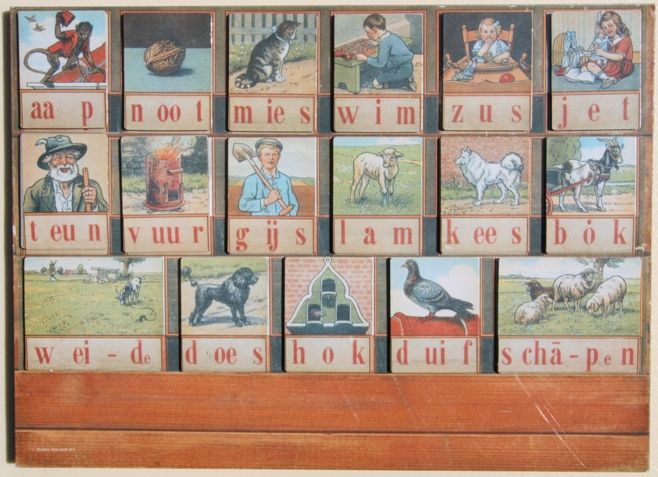
\includegraphics[width=0.5\linewidth]{graphics/leesplankje} 

}

\caption{Hoogeveen's Leesplankje.}\label{fig:hoogeveenjpg}
\end{figure}

For our stimulus set we selected the five humans Wim, Zus, Jet, Teun, Gijs.
Starting smacofMakeAllPairs() generates a sequence of tetrads on stdout,
giving the subject an opportunity to choose the most similar pair (or to
decide that both pairs are equally similar). On stdout we see (with responses)

\begin{Shaded}
\begin{Highlighting}[]
\SpecialCharTok{\textgreater{}} \FunctionTok{smacofMakeAllPairs}\NormalTok{(names)}
\NormalTok{(Gijs,Teun) }\FunctionTok{and}\NormalTok{ (Gijs,Wim)}
\NormalTok{most similar pair}\SpecialCharTok{:} \DecValTok{2}
\NormalTok{(Teun,Wim) }\FunctionTok{and}\NormalTok{ (Gijs,Jet)}
\NormalTok{most similar pair}\SpecialCharTok{:} \DecValTok{2}
\NormalTok{(Gijs,Zus) }\FunctionTok{and}\NormalTok{ (Jet,Zus)}
\NormalTok{most similar pair}\SpecialCharTok{:} \DecValTok{2}
\NormalTok{(Wim,Jet) }\FunctionTok{and}\NormalTok{ (Gijs,Wim)}
\NormalTok{most similar pair}\SpecialCharTok{:} \DecValTok{1}
\NormalTok{(Teun,Zus) }\FunctionTok{and}\NormalTok{ (Teun,Jet)}
\NormalTok{most similar pair}\SpecialCharTok{:}
\end{Highlighting}
\end{Shaded}

At the same time the same pairs are show on the graphics device, in the form shown in figure \ref{fig:hoogeveenpng}.

\begin{figure}

{\centering 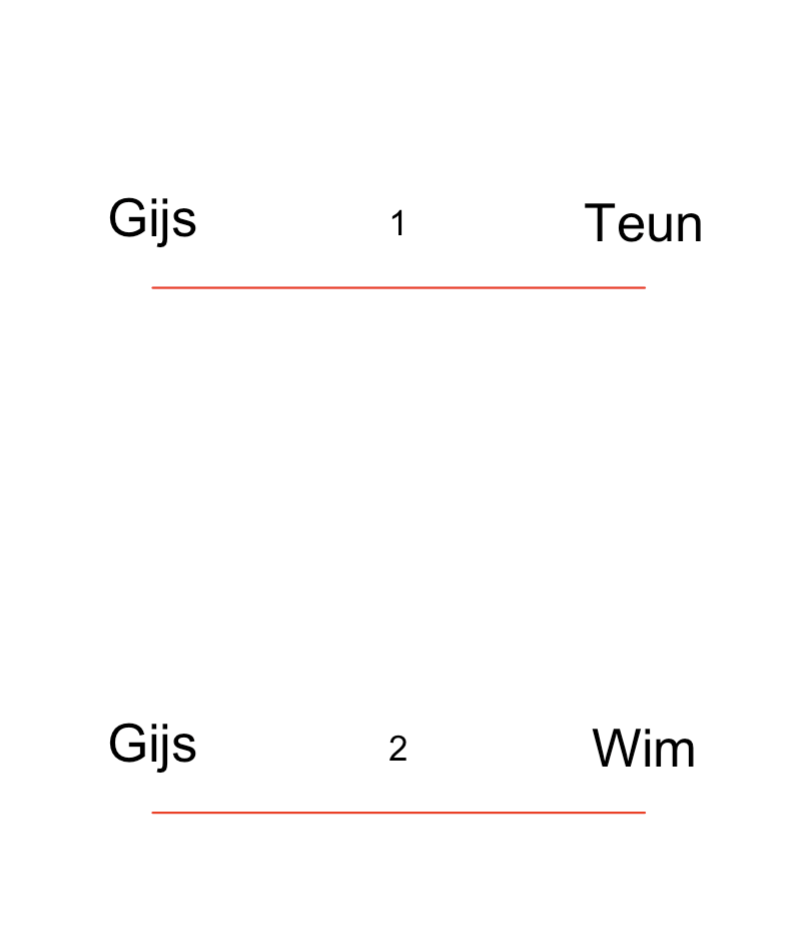
\includegraphics[width=0.3\linewidth]{graphics/hoogeveen} 

}

\caption{A Tetrad}\label{fig:hoogeveenpng}
\end{figure}

This continues until all tetrads are shown (in the case of
smacofMakeAllPairs()) or a given number of random pairs (without
replacement) has been shown (in the case of smacofMakeRandomPairs()).

As we discussed in the introduction smacofPC() is not limited to data
collected as tetrads. After suitable manipulation it can also
handle data collected by the method of triads or by conditional or complete
rank orders. In particular if we have a matrix of
dissimilarities between \(n\) objects we can convert it to a large number of comparisons of tetrads. This is done by the function
\texttt{smacofMakePairsFromDelta\ \textless{}-\ function(delta,\ ties\ =\ 1)}.

Alternatively we can code the order of dissimilarities using only
\(\binom{n}{2}-1\) tetrads, by using only those pairs that are
consecutive in the ordering of pairs. This is done by
\texttt{smacofOrderPairsFromDelta\ \textless{}-\ function(delta,\ ties\ =\ 1)}.

\subsection{Plots}\label{plots}

smacofPC does not have a Shepard plot, because there are no
dissimilarities to put on the horizontal axes. We do have

\begin{Shaded}
\begin{Highlighting}[]
\NormalTok{smacofConfigurationPlot }\OtherTok{\textless{}{-}}
  \ControlFlowTok{function}\NormalTok{(h,}
           \AttributeTok{main =} \StringTok{"ConfigurationPlot"}\NormalTok{,}
           \AttributeTok{dim1 =} \DecValTok{1}\NormalTok{,}
           \AttributeTok{dim2 =} \DecValTok{2}\NormalTok{,}
           \AttributeTok{pch =} \DecValTok{16}\NormalTok{,}
           \AttributeTok{col =} \StringTok{"RED"}\NormalTok{,}
           \AttributeTok{cex =} \FloatTok{1.0}\NormalTok{)}
\end{Highlighting}
\end{Shaded}

and

\begin{Shaded}
\begin{Highlighting}[]
\NormalTok{smacofDistDhatPlot }\OtherTok{\textless{}{-}} \ControlFlowTok{function}\NormalTok{(h,}
                               \AttributeTok{fitlines =} \ConstantTok{TRUE}\NormalTok{,}
                               \AttributeTok{colline =} \StringTok{"RED"}\NormalTok{,}
                               \AttributeTok{colpoint =} \StringTok{"BLUE"}\NormalTok{,}
                               \AttributeTok{main =} \StringTok{"Dist{-}Dhat Plot"}\NormalTok{,}
                               \AttributeTok{cex =} \FloatTok{1.0}\NormalTok{,}
                               \AttributeTok{lwd =} \DecValTok{2}\NormalTok{,}
                               \AttributeTok{pch =} \DecValTok{16}\NormalTok{)}
\end{Highlighting}
\end{Shaded}

\section{Examples}\label{examples}

\subsection{Hoogeveen}\label{hoogeveen}

A single subject (me) ran smacofMakeAllPairs() on the five leesplankje names. This
produced 45 tetrads.

Convergence is to stress \ensuremath{3.1647986\times 10^{-9}} in 296 iterations. The curved solution
Teun-Gijs-Wim-Jet-Zus goes from old-male to young-female. The 45 inequalities
in the data can be satisfied exactly.

\begin{greybox}

\begin{center}
\textbf{INSERT FIGURE \ref{fig:hoogeconf} ABOUT HERE}

\end{center}

\end{greybox}

\begin{greybox}

\begin{center}
\textbf{INSERT FIGURE \ref{fig:hoogedd} ABOUT HERE}

\end{center}

\end{greybox}

\subsection{Parties}\label{parties}

I left The Netherlands in 1987 and have not followed their local political news. So I am not really an expert on current Dutch politics. Nevertheless I was the only subject generating the data (50 random tetrads) for this example. The ten parties I used are

\begin{itemize}
\tightlist
\item
  SP Socialists
\item
  GL Greens
\item
  PvdD Party for the Animals
\item
  PvdA Labour
\item
  D'66 Neither fish nor fowl
\item
  CDA Christian Democrats
\item
  VVD European-style Liberals
\item
  CU More Christian Democrats
\item
  SGP Right-wing Christians
\item
  FVD Right-wing Populists
\end{itemize}

For more details, see this \href{https://en.wikipedia.org/wiki/List_of_political_parties_in_the_Netherlands}{Wikipedia article}.

Convergence is to stress \ensuremath{1.1150739\times 10^{-9}} in 135 iterations. The solution is
in an almost equilateral triangle with the three extremes (FVD, SP, SGP) in the
vertices. The interior of the triangle shows a social democratic (PvdA, PvdD, GL),
a liberal (VVD, D'66), and a christian democrat (ARP, CU, CDA) cluster,
roughly ordered from left-wing on the right of the plot to right-wing on the left of the plot. Again, all 50 inequalities can be fitted exactly.

We can check how sparse and balanced the randomly generated ``design'' is by printing the \(\epsilon_{ij}^\star\).

\begin{verbatim}
##       [,1] [,2] [,3] [,4] [,5] [,6] [,7] [,8] [,9] [,10]
##  [1,]    0    2    3    3    2    4    2    1    0     2
##  [2,]    2    0    2    3    1    2    1    4    3     1
##  [3,]    3    2    0    3    3    3    4    2    1     0
##  [4,]    3    3    3    0    0    3    1    4    4     2
##  [5,]    2    1    3    0    0    2    0    3    2     6
##  [6,]    4    2    3    3    2    0    2    0    4     5
##  [7,]    2    1    4    1    0    2    0    1    2     1
##  [8,]    1    4    2    4    3    0    1    0    2     2
##  [9,]    0    3    1    4    2    4    2    2    0     2
## [10,]    2    1    0    2    6    5    1    2    2     0
\end{verbatim}

with row sums 19, 19, 21, 23, 19, 25, 14, 19, 20, 21. For an all-pairs-of-pairs design the
elements of this matrix would have been 44. So the random
``design'' is very sparse but decently balanced.

\begin{greybox}

\begin{center}
\textbf{INSERT FIGURE \ref{fig:partiesconf} ABOUT HERE}

\end{center}

\end{greybox}

\begin{greybox}

\begin{center}
\textbf{INSERT FIGURE \ref{fig:partiesdd} ABOUT HERE}

\end{center}

\end{greybox}

\subsection{Ekman (1954)}\label{ekman_54}

The ekman data are dissimilarities between 14 colors. This means they can be
expanded into 4095 tetrads, which can then be
analyzed by smacofPC(). We do not necessarily recommend this practice, because
the pairwise coding involves a great deal of dependence and redundancy.
The smacofPC() program is really intended for sequences of independent tetrads judgments. Nevertheless we will use these expanded ekman dissimilarities as an example.

Convergence is to stress 0.0087145 in 82 iterations. The solution is the
familiar color circle, except that, for some reason that I do not understand yet, the circle is crumpled at the high frequency
end.

\begin{greybox}

\begin{center}
\textbf{INSERT FIGURE \ref{fig:ekmanconf} ABOUT HERE}

\end{center}

\end{greybox}

\begin{greybox}

\begin{center}
\textbf{INSERT FIGURE \ref{fig:ekmandd} ABOUT HERE}

\end{center}

\end{greybox}

\section{Figures}\label{figures}

\begin{figure}

{\centering 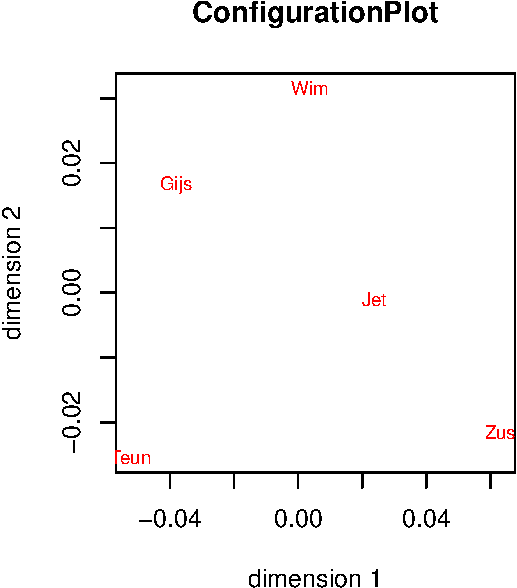
\includegraphics{smacofPC_files/figure-latex/hoogeconf-1} 

}

\caption{Leesplankje}\label{fig:hoogeconf}
\end{figure}

\begin{figure}

{\centering 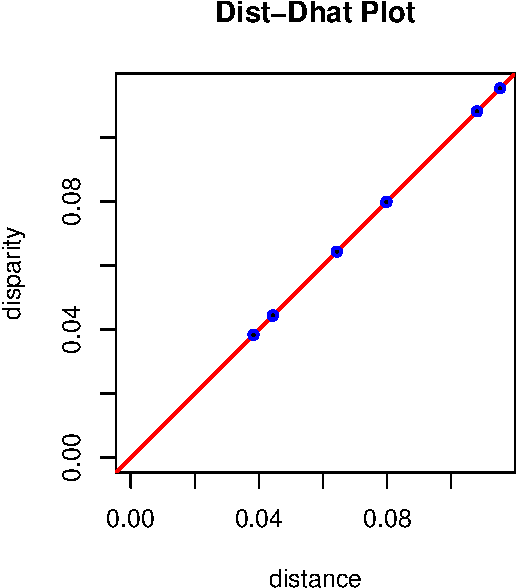
\includegraphics{smacofPC_files/figure-latex/hoogedd-1} 

}

\caption{Leesplankje}\label{fig:hoogedd}
\end{figure}

\begin{figure}

{\centering 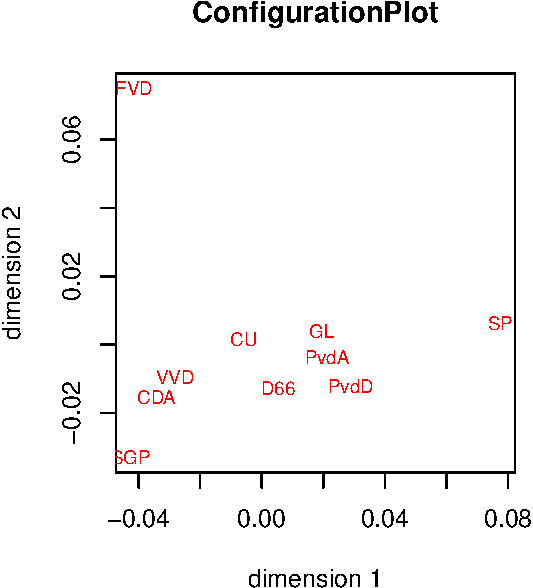
\includegraphics{smacofPC_files/figure-latex/partiesconf-1} 

}

\caption{Dutch political parties}\label{fig:partiesconf}
\end{figure}

\begin{figure}

{\centering 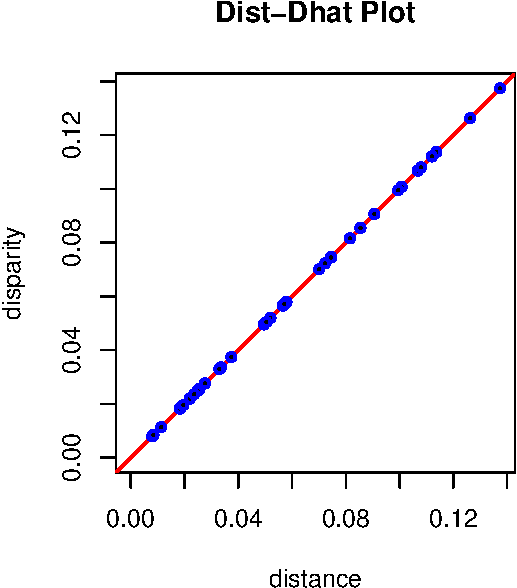
\includegraphics{smacofPC_files/figure-latex/partiesdd-1} 

}

\caption{Dutch political parties}\label{fig:partiesdd}
\end{figure}

\begin{figure}

{\centering 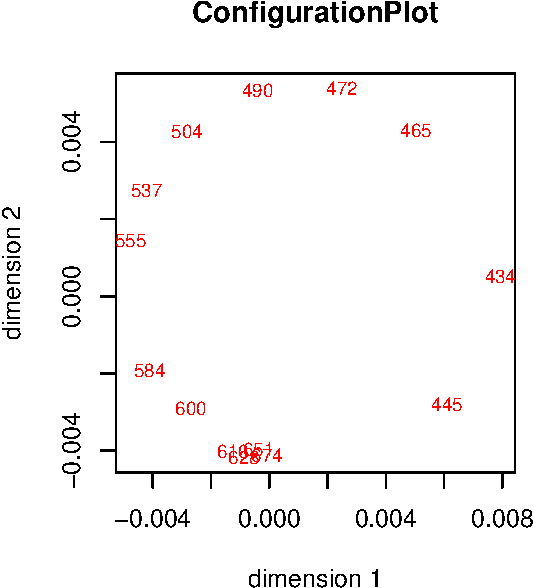
\includegraphics{smacofPC_files/figure-latex/ekmanconf-1} 

}

\caption{Ekman color data}\label{fig:ekmanconf}
\end{figure}

\begin{figure}

{\centering 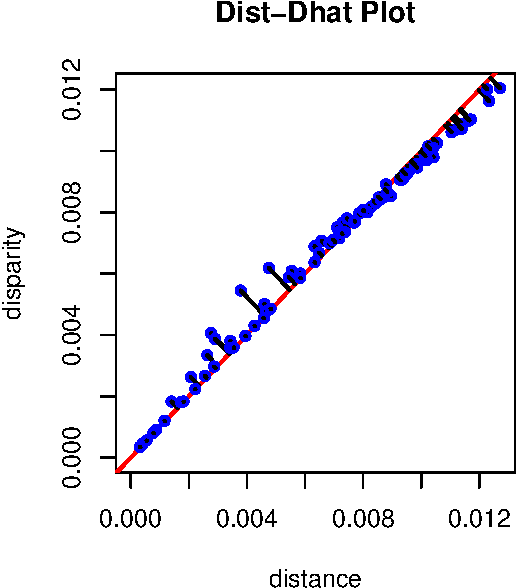
\includegraphics{smacofPC_files/figure-latex/ekmandd-1} 

}

\caption{Ekman color data}\label{fig:ekmandd}
\end{figure}

\section*{References}\label{references}
\addcontentsline{toc}{section}{References}

\phantomsection\label{refs}
\begin{CSLReferences}{1}{0}
\bibitem[\citeproctext]{ref-agarwal_wills_cayton_lanckriet_kriegman_belongie_07}
Agarwal, S., J. Wills, L. Cayton, G. Lanckriet, D. Kriegman, and S. Belongie. 2007. {``Generalized Non-Metric Multidimensional Scaling.''} In \emph{Proceedings of the Eleventh International Conference on Artificial Intelligence and Statistics}, 11--18.

\bibitem[\citeproctext]{ref-coombs_54}
Coombs, C. H. 1954. {``A Method for the Study of Interstimulus Similarity.''} \emph{Psychometrika} 19: 183--94.

\bibitem[\citeproctext]{ref-deleeuw_R_68g}
De Leeuw, J. 1968. {``Nonmetric Multidimensional Scaling.''} Research Note 010-68. Department of Data Theory FSW/RUL. \url{https://jansweb.netlify.app/publication/deleeuw-r-68-9/deleeuw-r-68-g.pdf}.

\bibitem[\citeproctext]{ref-deleeuw_R_70a}
---------. 1970. {``The Positive Orthant Method for Nonmetric Multidimensional Scaling.''} Research Report 001-70. Leiden, The Netherlands: Department of Data Theory FSW/RUL. \url{https://jansweb.netlify.app/publication/deleeuw-r-70-a/deleeuw-r-70-a.pdf}.

\bibitem[\citeproctext]{ref-deleeuw_B_73}
---------. 1973. {``Canonical Analysis of Categorical Data.''} PhD thesis, University of Leiden, The Netherlands. \url{https://jansweb.netlify.app/publication/deleeuw-b-73/deleeuw-b-73.pdf}.

\bibitem[\citeproctext]{ref-deleeuw_U_75a}
---------. 1975. {``{A Normalized Cone Regression Approach to Alternating Least Squares Algorithms}.''} Department of Data Theory FSW/RUL.

\bibitem[\citeproctext]{ref-deleeuw_B_84}
---------. 1984. \emph{Canonical Analysis of Categorical Data}. Leiden, The Netherlands: DSWO Press. \url{https://jansweb.netlify.app/publication/deleeuw-b-84/deleeuw-b-84.pdf}.

\bibitem[\citeproctext]{ref-deleeuw_E_18d}
---------. 2018. {``{The Positive Orthant Method }.''} 2018. \url{https://jansweb.netlify.app/publication/deleeuw-e-18-d/deleeuw-e-18-d.pdf}.

\bibitem[\citeproctext]{ref-ekman_54}
Ekman, G. 1954. {``{Dimensions of Color Vision}.''} \emph{Journal of Psychology} 38: 467--74.

\bibitem[\citeproctext]{ref-guttman_46}
Guttman, L. 1946. {``{An Approach for Quantifying Paired Comparisons and Rank Order}.''} \emph{Annals of Mathematical Statistics} 17: 144--63.

\bibitem[\citeproctext]{ref-guttman_69}
---------. 1969. {``{Smallest Space Analysis by the Absolute Value Principle}.''} In \emph{{Proceedings of the XIX International Congress of Psychology, London}}.

\bibitem[\citeproctext]{ref-guttman_79}
---------. 1979. {``Smallest Space Analysis by the Absolute Value Principle.''} In \emph{{Geometric Representations of Relational Data}}, edited by J. C. Lingoes, E. E. Roskam, and I. Borg, 707--12. Mathesis Press.

\bibitem[\citeproctext]{ref-hartmann_79}
Hartmann, W. 1979. \emph{{Geometrische Modelle zur Analyse empirischer Data}}. Akademie Verlag.

\bibitem[\citeproctext]{ref-hayashi_52}
Hayashi, C. 1952. {``On the Prediction of Phenomena from Qualitative Data and the Quantification of Qualitative Data from the Mathematico-Statistical Point of View.''} \emph{Annals of the Institute of Statistical Mathematics} 3: 69--98.

\bibitem[\citeproctext]{ref-johnson_73}
Johnson, R. M. 1973. {``{Pairwise Nonmetric Multidimensional Scaling}.''} \emph{Psychometrika} 38 (12--18).

\bibitem[\citeproctext]{ref-kruskal_carroll_69}
Kruskal, J. B., and J. D. Carroll. 1969. {``{Geometrical Models and Badness of Fit Functions}.''} In \emph{Multivariate Analysis, Volume II}, edited by P. R. Krishnaiah, 639--71. North Holland Publishing Company.

\bibitem[\citeproctext]{ref-okamoto_isogai_78}
Okamoto, M., and T. Isogai. 1978. {``Optimality of Multidimensional Representation in Hayashi's Fourth Method of Quantification.''} \emph{Journal of the Japanese Statistical Society} 8 (2): 63--69.

\bibitem[\citeproctext]{ref-roskam_70}
Roskam, E. E. 1970. {``The Method of Triads for Nonmetric Multidimensional Scaling.''} \emph{Nederlands Tijdschrift Voor de Psychologie} 25 (404-417).

\bibitem[\citeproctext]{ref-roskam_79b}
---------. 1979. {``The Method of Triads for Nonmetric Multidimensional Scaling.''} In \emph{{Geometric Representations of Relational Data}}, edited by J. C. Lingoes, E. E. Roskam, and I. Borg, 497--509. Mathesis Press.

\bibitem[\citeproctext]{ref-takane_78b}
Takane, Y. 1978a. {``A Maximum Likelihood Method for Nonmetric Multidimensional Scaling: I. The Case in Which All Empirical Pairwise Orderings Are Independent - Evaluations.''} \emph{Japanese Psychological Research} 20 (3): 105--14.

\bibitem[\citeproctext]{ref-takane_78a}
---------. 1978b. {``A Maximum Likelihood Method for Nonmetric Multidimensional Scaling: I. The Case in Which All Empirical Pairwise Orderings Are Independent - Theory.''} \emph{Japanese Psychological Research} 20 (1): 7--17.

\bibitem[\citeproctext]{ref-torgerson_58}
Torgerson, W. S. 1958. \emph{{Theory and Methods of Scaling}}. New York: Wiley.

\end{CSLReferences}

\end{document}
